%
% The MIT License (MIT)
%
% Copyright (c) 2016 Paul Batty
%
% Permission is hereby granted, free of charge, to any person obtaining a copy
% of this software and associated documentation files (the "Software"), to deal
% in the Software without restriction, including without limitation the rights
% to use, copy, modify, merge, publish, distribute, sublicense, and/or sell
% copies of the Software, and to permit persons to whom the Software is
% furnished to do so, subject to the following conditions:
%
% The above copyright notice and this permission notice shall be included in
% all copies or substantial portions of the Software.
%
% THE SOFTWARE IS PROVIDED "AS IS", WITHOUT WARRANTY OF ANY KIND, EXPRESS OR
% IMPLIED, INCLUDING BUT NOT LIMITED TO THE WARRANTIES OF MERCHANTABILITY,
% FITNESS FOR A PARTICULAR PURPOSE AND NONINFRINGEMENT. IN NO EVENT SHALL THE
% AUTHORS OR COPYRIGHT HOLDERS BE LIABLE FOR ANY CLAIM, DAMAGES OR OTHER
% LIABILITY, WHETHER IN AN ACTION OF CONTRACT, TORT OR OTHERWISE, ARISING FROM,
% OUT OF OR IN CONNECTION WITH THE SOFTWARE OR THE USE OR OTHER DEALINGS IN
% THE SOFTWARE.
%

\section{Background}
\label{sec:sqlite_intro}

The following chapter will cover two completely different programs that operate on SQLite. Then look towards SQLite's beginnings, and where it is used. Starting back in spring of 2000. Finishing off with a look at the SQLite file format. Before moving onto the other sections.

\subsection{Similar programs}
\label{subsec:similar_programs}

While searching the web for tools only two different types appeared. The graphical interface. They would provide a graphical user interface into SQLite, removing the need for using SQL and the command line directly. Or very technical tools, and no middle ground. This was particularly interesting as the number of user interface tools completely outnumbered the technical tools, where only one could be found.

\subsubsection{SQLite browser}
\label{subsubsec:sqlite_browser}

The first tool, SQLite browser, made by \cite{sqlitebrowser} based off of the Arca database browser. Out of all the user interface tools out there this was the most polished. It allowed users to open, view and manipulate the database. Without having to learn SQL or the command line. With the main aim to be as simple as possible. Below figure~\ref{fig:db_browser_screen} shows a screen shot of the program.

\begin{figure}[H]
	\centering
	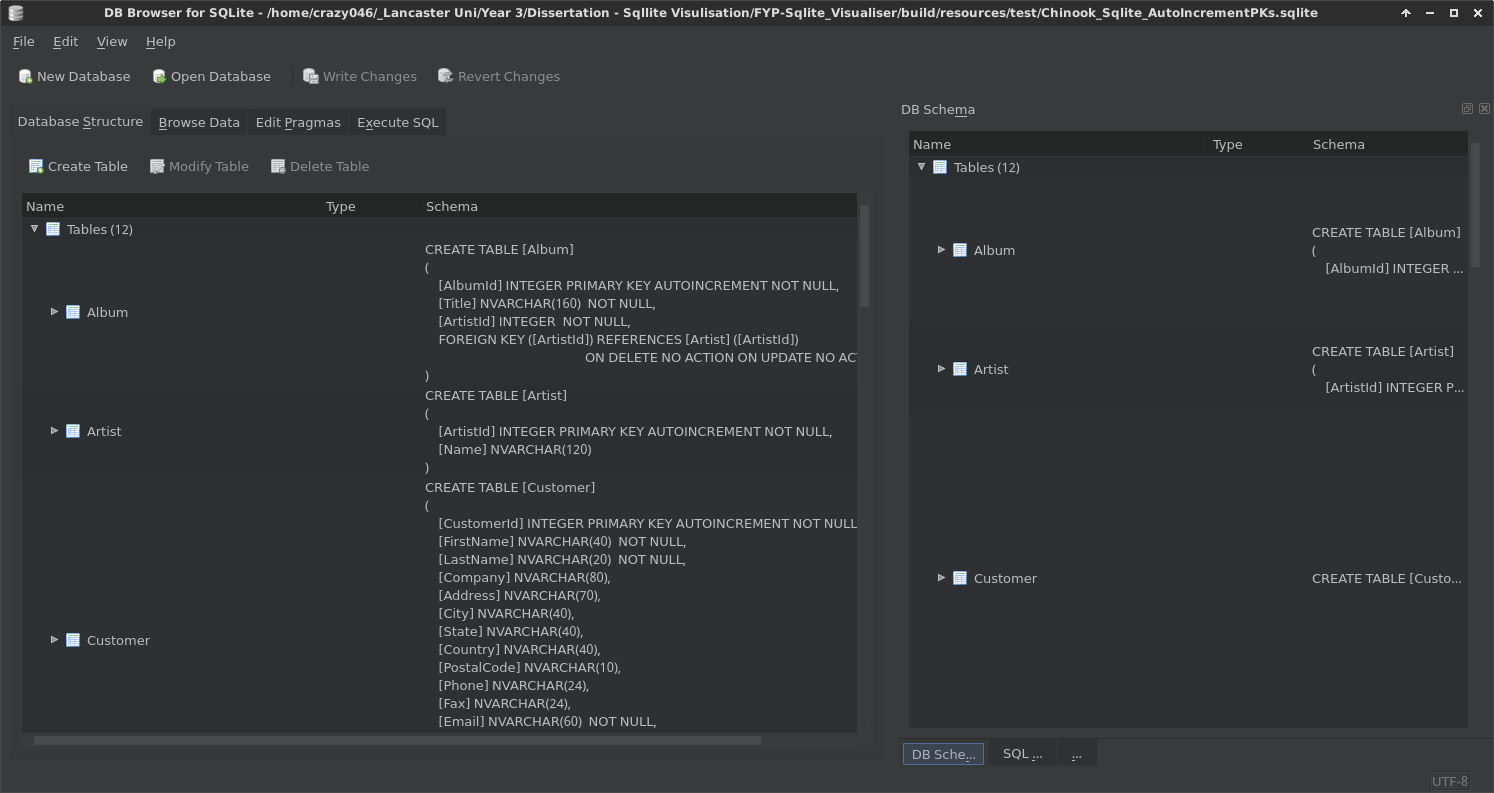
\includegraphics[scale=0.25]{images/db_browser.png}
	\caption{Screen shot of the SQLite database browser.}
	\label{fig:db_browser_screen}
\end{figure}

Apart from the usual features, such as viewing tables, schemas, and modifying them. The more unique features allowed exporting the tables to CSV (comma separated values), producing SQL dumps and acting as a sandbox. The sandbox allowed users to execute commands, see the changes, but nothing was actually performed until the user committed the changes onto the database. In addition  to this it provided a fully fledged SQL editor with auto-complete, syntax highlighting and loading and saving of commands in external files.
\\\\
The tool itself was made in C/C++ and QT, with support for SQLite databases up to version 3.8.2. It is available for all major platforms. The user interface and features built into the tool where simple and intuitive to navigate. It was very powerful and can be very usefully to anyone working with SQLite that does not want to use the command line. However, it did not allow an insight into SQLite nor the logging of commands, produced by external programs.

\subsubsection{SQLite fragmentation}
\label{subsubsec:sqlite_fragmentation}

The second tool is unique. It showed a fragmented view of the database. Made by \cite{sqlitefrag}. Written in python and published to Github. It only did one thing but did it well. As mentioned later later on, the file format is made up of pages. This tool would scan the file, and produce a visualisation of the fragmentation status of each page. Much like that old Windows 98 de-fragmentation tool. See figure~\ref{fig:db_visualizer} for a screen shot.

\begin{figure}[H]
	\centering
	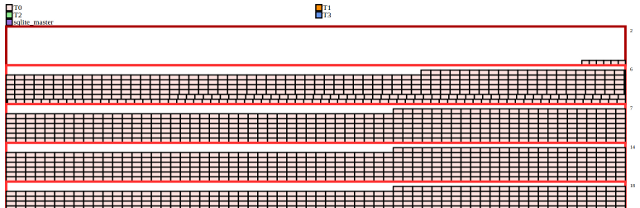
\includegraphics[scale=0.85]{images/db_visualizer.png}
	\caption{Screen shot of the SQLite fragmentation visualiser. \citep{sqlitefrag}}
	\label{fig:db_visualizer}
\end{figure}

The tool runs though the command line, and produces a JSon file with the analysis, before sending it to the visualiser that produces a SVG image output. This allows any type of output to be added in. Some of the more advanced features allow filtering certain pages out or in, and de-fragmentation. 
\\\\
Although it is very powerful, it does not support WAL mode, slow on larger databases and can only cope with UTF-8 text support. WAL mode, or write ahead logging, is an alternative to a rollback journal, where the changes are written to the log. This log is then inserted into the database file at each checkpoint during the transaction. The rollback journal takes the opposite approach and changes the database with the journal holding the backup. Overall, this tool provides a very useful insight into SQLite. On top of this, it clearly shows the page format of the file, which is very similar to where my tool is going.

\subsection{What is SQLite}
\label{subsec:what_is_sqlite}

D. Richard Hipp, the author of SQLite, Originally got the idea while working on a battleship. He was tasked with developing a program for the on board guided missiles. While working on the software he used the database system Informix. Which took hours to set up and get anywhere near useful. For the application that he was building, all he needed was a small self-contained, portable and easy to use database. Rather than such a large, all powerful system. \citep{sqlitedefguide}.
\\\\
Speaking to a colleague in January of 2000, Hipp, disused his idea for a self contained embedded database. When some free time opened up on the 29th of May 2000, SQLite was born. It was not until August 2000 that version 1.0 was released. Then in just over a year on the 28 November 2001, 2.0 which introduced, B-Trees and many of the features seen in 3.0 today. During the next year he joined up with Joe Mistachkin followed by Dan Kennedy in 2002. To help work for the 3.0 release, which came a lot later containing a full rewrite and improvements over 2.0, with the first public release on 18 June 2004. At the time of writing this paper the current version of SQLite is 3.10.4. After changes to the naming scheme, version 3 is currently supported to 2050. \citep{sqlite}.
\\\\
Today, SQLite is open source within the public domain making it accessible to everyone. The entire library size is around 350Kib, with some optional features omitted it could be reduced to around 300Kib making it incredibly small compared to what it does. In addition to this the runtime usage is minimal with 4Kib stack space and 100Kib heap, allowing it to run on almost anything. SQLite's main strength is that the entire database in encoded into a single portable file, that can be read, on any system whether 32 or 64 bit, big or small endian. It is often seen as a replacement for storage files rather than a database system. In fact Hipp (2000) stated, "Think of SQLite not as a replacement for Oracle but as a replacement for fopen()".

\subsection{Where is SQLite used}
\label{subsec:where_is_sqlite}

SQLite being a relational database engine, as well as a replacement for fopen() \citep{sqlite}. Allows it to be truly used for anything. Hipp has stated numerous times that SQLite might be the single most deployed software currently. Alongside zlib, libpng and libjpg. With the numbers in the billions and billions \citep{sqlite}.
\\\\
This large distribution means SQLite can be found anywhere. Microsoft even approached Hipp, and asked for a special version to be made for use in Windows 10 \citep{sqlitetalk}. In addition to Microsoft. Apple, Google and Facebook all use SQLite, somewhere within their systems. On top of all the big names. You can find it, within any another consumer device, such as Phones, Cameras and Televisions. This wide usage was picked up by Google and Hipp was awarded “Best Integrator” at O’Reilly’s 2005 Open Source Convention \citep{sqlitedefguide}. 

\subsection{How SQLite works}
\label{subsec:how_sqlite_works}

SQLite has a simple and very modular design. Consisting of eleven modules, and four subsystems. The backend, The core, The SQL compiler, and Accessories. Figure~\ref{fig:sqlite_arch} shows the architectural diagram of SQLite.

\begin{figure}[H]
	\centering
	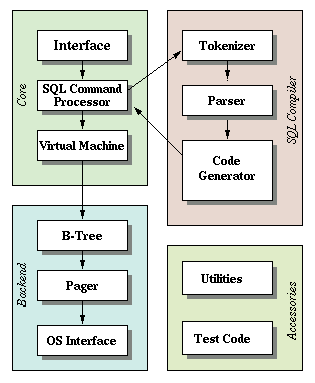
\includegraphics[scale=0.50]{images/sqlite_arch.png}
	\caption{Sqlite architectural diagram \citep{sqlite}}
	\label{fig:sqlite_arch}
\end{figure}

\subsubsection{The SQL Compiler}
\label{subsec:how_sqlite_compiler}

The SQL compiler takes SQL strings and converts them into the core's virtual machine assembly language. The process starts with the tokenizer and parser. They both work closely together. Taking the SQL string and validating the syntax. Before converting it into a hierarchical structure for use by the code generator. Both systems are custom made for SQLite. With the parser going under the name of Lemon \citep{sqlitedefguide}. Lemon is designed to optimise performance and guard against memory leaks. Once they have successfully converted the SQL string into a Parse Tree, the parser passes it onto the code generator.
\\\\
The code generator takes the parse tree from the parser, and translates it into an assembly language program. The program is written in a assembly language that is specifically designed for SQLite. It is run by the virtual machine inside the core module. Once the assembly program is constructed it is sent to the virtual machine for execution.

\subsubsection{The Core}
\label{subsec:how_sqlite_core}

The Core itself is actually one single virtual machine implementing a specifically designed computing engine to manipulate database files. The language contains 128 instructions, all designed to manipulate and interact with the database, or prepare the machine for such operations. Figure~\ref{fig:vm_code} shown an example program. 
\begin{figure}[H]
	\centering
	\begin{lstlisting} 
		SQL =  SELECT * FROM examp;
		addr  opcode        p1     p2     p3                                 
		----  ------------  -----  -----  ---------------------
		0     ColumnName    0      0      one                                
		1     ColumnName    1      0      two                                
		2     Integer       0      0                                         
		3     OpenRead      0      3      examp                              
		4     VerifyCookie  0      81                                        
		5     Rewind        0      10                                        
		6     Column        0      0                                         
		7     Column        0      1                                         
		8     Callback      2      0                                         
		9     Next          0      6                                         
		10    Close         0      0                                         
		11    Halt          0      0
	\end{lstlisting}
	\caption{Select operation program from \cite{sqlite}}
	\label{fig:vm_code}
\end{figure}

The interface module defines the interface between the virtual machine and the SQL library. All libraries and external application use this to communicate with SQLite.
\\\\
With this in mind the virtual machine takes the SQL input from the Interface, passes it onto the SQL Compiler. Then collecting the resulting program from the code generator, and executing this program to perform the original request that was sent in. Making it the heart or core of SQLite's operations.

\subsubsection{The Backend}
\label{subsec:how_sqlite_backend}

The final main module is the backend. It deals with the file interactions, such as writing, reading and ordering of the file. The B-Tree and pager work closely together to organise the pages, both of which do not care what the page contains. The B-Tree module is like a factory that maintains and sorts the relationships between each of the different pages within the file. Forming them into a tree structure that makes it easy to find what you are after. 
\\\\
The OS Interface is a warehouse, providing a constant interface to the disk. It handles the locking, reading and writing of files across all types of operating systems. So the pager does not have to worry about how it is implemented, it can just tell it what it wants.
\\\\
Lastly, the Pager is the transport truck, going between the B-Tree (factory) and the OS interface (storage) to deliver pages at the B-tree requests. It also keeps the most commonly used pages in its cache, so it does not have to keep going through the OS interface in order to collect the pages, since it already has them.

\subsubsection{The Accessories}
\label{subsec:how_sqlite_accessories}

The last module, accessories is made up of two parts, utility and tests. The utility module contains functions that are used all across SQLite, such as memory allocation, string comparison, random number generator and symbol tables. This basically acts as a shared system for all parts of SQLite. The test section contains all the test scripts and only exists for testing purposes, of which contains over 811 times more code then the actual project and millions of test cases. As it covers every possible code path through SQLite. This is partly why SQLite is considered to be so reliable. 
\\\\
\subsection{The SQLite file format}
\label{subsec:sqlite_file_format}

\subsubsection{The page system}
\label{subsubsec:sqlite_page_system}

As mentioned in section~\ref{subsec:how_sqlite_backend} the B-Tree module looks after the pages including the organisation and relationships between them. Packing them into a tree structure. This is the same structure that gets written to disk. The B-Tree implementation is designed to support fast querying. The various B-Tree structures can be found in \cite{btreepaper} The ubiquitous B-Tree paper. SQLite also takes some improvements seen in \cite{btreeimprpaper} Sorting and searching book \citep{sqliteray}.
\\\\
The basic idea is that the file is made up of pages, each page is the same fixed size. The size of the pages are a power of two between 512 - 65536 bytes. Pages are numbered starting with 1 instead of 0. The maximum number of pages that Sqlite can hold is 2,147,483,646 with a page size of 512 bytes or around 140 terabytes. The minimum number of pages within a database is 1. There are five types of pages:

\begin{itemize} 
	\item Lock Byte Page \hfill \\
		The lock byte page appears between bytes, 1073741824 - 1073742335, if a database is smaller or equal to 1073742335 bytes it will not contain a lock byte page. It is used by the operating system not SQLite.
	
	\item Freelist Page \hfill \\
		The freelist page is an unused page, often left behind when information is deleted from the database. The other type is a freelist trunk page containing page numbers of the other freelist pages.
	
	\item B-Tree Page \hfill \\
		The B-Tree page contains one of the four types of B-Trees, more in section~\ref{subsubsec:sqlite_trees_and_cells}.
	
	\item Payload overflow page \hfill \\
		The payload overflow page is created to hold the remaining payload from a B-Tree cell when the payload is too large.
	
	\item Pointer map page \hfill \\
		Pointer map pages are inserted to make the vacuum modes faster. And is the reverse B-Tree going child to parent rather than parent to child. They exist in databases that have a non-zero value largest root B-Tree within the header. The first instance of these pages are at page 2. 
\end{itemize} 

This paper will not cover the lock byte and pointer map pages. 
\\\\
\subsubsection{The Header}
\label{subsubsec:sqlite_page_hader}

The first step in parsing the SQLite file before the different pages is to read in the SQLite header. This is the first 100 bytes located in page one. The header stores all the necessary information to read the rest of the file. So reading it correctly is crucial. Immediately following the header is the root B-Tree which is covered in the next section. Appendix A shows the full header layout.
\\
\subsubsection{The Trees and Cells}
\label{subsubsec:sqlite_trees_and_cells}

As mentioned in section~\ref{subsubsec:sqlite_page_system} the file is split into pages and each page contains one of five types of pages. However, each page is linked together in a B-Tree format, where each page represents a node in the tree. Below figure~\ref{fig:sqlite_btree_figure} shows an example file B-Tree.

\begin{figure}[H]
	\centering
	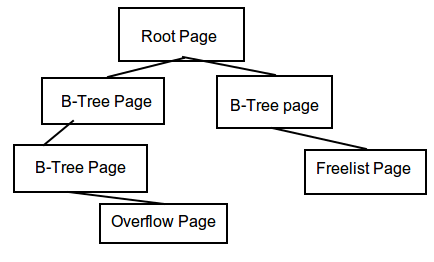
\includegraphics[scale=0.5]{images/sqlite_btree_format.png}
	\caption{B-Tree page structure.}
	\label{fig:sqlite_btree_figure}
\end{figure}

One thing to note is how the file is made up of mainly B-Tree pages. This is briefly mentioned in the last section, where pointer maps, lock byte and overflow pages only appear when the requirements are met. And Freelist page when enough data has been deleted. Leaving only the B-Tree pages.
\\\\
At the start of each B-Tree page there is the B-Tree / page header. Following the header is an array of pointers to their cells. One thing to note is that the first page also has the database header. This mean you will have to skip it before reaching the page header. Figure~\ref{fig:sqlite_file_format} shows the full layout of the SQLite file.

\begin{figure}[H]
	\centering
	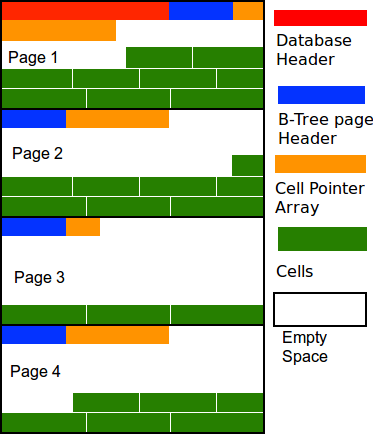
\includegraphics[scale=0.5]{images/sqlite_file_format.png}
	\caption{Sqlite file format, modified from \cite{sausagefactory}}
	\label{fig:sqlite_file_format}
\end{figure}

When the cells are added to the page, they start at the end of the page and work backwards towards the top. The main difference between each type of B-tree page can be seen inside the cells as they carry the payload for the node. 
\\\\
As mentioned in section~\ref{subsubsec:sqlite_page_system} there are four types of B-Trees. These can be split into two main types, and two sub types. The main types are Table and Index, both of which uses a key-value system in order to organise them. The Table B-Trees use 64 bit integers also known as row-id or primary key, theses are often what the user has set inside the database, else SQLite will attach its own. The Index B-Trees use database records as keys. 
\\\\
The sub types of B-Trees are broken down into Leaf and Interior. The leaves are located at the end of the tree and contain no children. Whereas the interior will always have at least one single child. In addition to this all database records / values within the B-Trees are sorted using the following rules written by \cite{sqliteray}:

\begin{enumerate} 
	\item If both values are NULL, then they are considered equal.
	\item If one value is a NULL and the other is not, it is considered the lesser of the two.
	\item If both values are either real or integer values, then the comparison is done numerically.
	\item If one value is a real or integer value, and the other is a text or blob value, then the numeric value is considered lesser
	\item If both values are text, then the collation function is used to compare them. The collation function is a property of the index column in which the values are found
	\item If one value is text and the other a blob, the text value is considered lesser.
	\item If both values are blobs, memcmp() is used to determine the results of the comparison function. If one blob is a prefix of the other, the shorter blob is considered lesser. 
\end{enumerate}
  
Overall the four types of B-Trees found inside SQLite are:

\begin{itemize} 
	\item Index B-Tree Interior
	\item Index B-Tree leaf
	\item Table B-Tree Interior
	\item Table B-Tree leaf 
\end{itemize} 

In the case of index B-Trees, the interior trees contain \textit{N} children and \textit{N-1} database records where \textit{N} is two or greater. Whereas a leaf will always contain \textit{M} database records where \textit{M} is a one or greater. The database records stored inside an Index B-Tree are of the same quantity as the associated database table, with the same fields and columns, between the tables and rows. This can be seen in figure~\ref{fig:sqlite_key_pair}. Index trees are used by SQLite to keep track the foreign keys and row relationships.

\begin{lstlisting}
 CREATE TABLE t1(a INTEGER PRIMARY KEY, b, c, d);
 CREATE INDEX i1 ON t1(d, c);

 INSERT INTO t1 VALUES(1, 'triangle', 3, 180, 'green');
 INSERT INTO t1 VALUES(2, 'square',   4, 360, 'gold');
 INSERT INTO t1 VALUES(3, 'pentagon', 5, 540, 'grey');
\end{lstlisting}

\begin{figure}[H]the format.
	\centering
	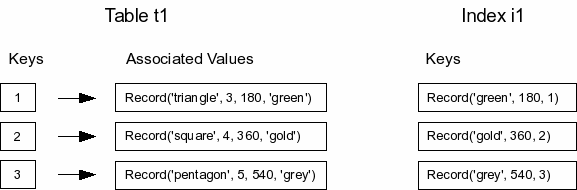
\includegraphics[scale=0.5]{images/examplepop.png}
	\caption{Example key pair database \citep{sqliteray}}
	\label{fig:sqlite_key_pair}
\end{figure}

The table B-Trees are completely different to the index trees. The interior type contains no data but only pointers to child B-Tree pages, as all the data is stored on the leaf type. The interior trees contain at least one pointer, and the leaf node contains at least one record. For each table that exists in the database, one corresponding Table B-Tree also exists, and that B-Tree contains one entry per row, appearing in the same order as the logical database. Figure~\ref{fig:sqlite_table_btree} shows the physical layout of the Table B-Tree. 

\begin{figure}[H]
	\centering
	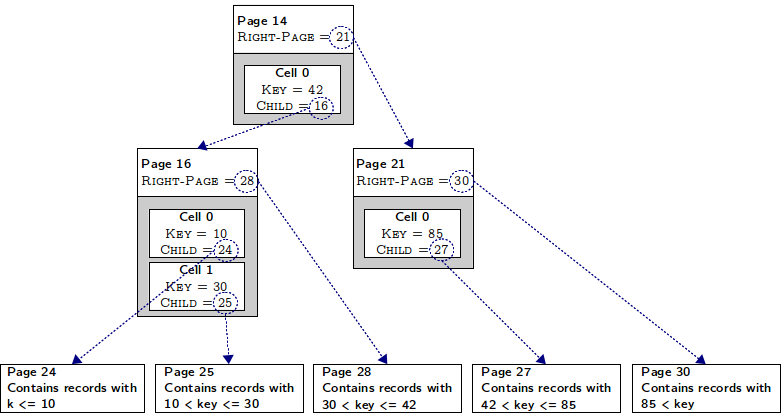
\includegraphics[scale=0.5]{images/sqlite_table_btree.png}
	\caption{Physical layout of table B-Trees \citep{chibd}}
	\label{fig:sqlite_table_btree}
\end{figure}

\subsubsection{Encoding of the data}
\label{subsubsec:sqlite_data_encoding}

SQLite uses a variable length integer or 'varint' in order to encode some of the values inside the database, since they use up less space for small positive values. A varint is a static Huffman encoding of a 64-bit two complements integer. Taking up between and 1 - 9 bytes in size. The maximum number a byte can hold is 127 as the most significant bit is needed as a flag unless it is the ninth byte where all the bits are used. If the most significant bit is set then the next byte is needed. So if it is set in byte 1 then byte 2 is needed and so on until, either the bit is not set, or the 9th byte is reached.
\\\\
For example, taking the following value in hex 5B and converting this to binary, creates the value 01011011, in this case the most significant bit is not set leaving the final value at 91. However, if the value in hex is 84 and converting this to binary creates the value 10000100, the most significant bit is set, therefore the next byte is needed. In this case the value of the next byte in hex is 60, converting this to binary creates  01100000 meaning that this varint is two byes long. In order to create the final value, the bytes need to be concatenated together leaving out the most significant bit. Creating the value 00001001100000 giving a final value of 608 in decimal \citep{sausagefactory}. Table~\ref{tbl:varints} shows  all combinations of varints. 

\begin{longtable}[h]{| c | c | p{10cm} |}
		\hline
			\textbf{Bytes} & \textbf{Value Range} & \textbf{Bit pattern} \\ 
		\hline
		\endhead
			1 & 7 &  0xxxxxxx \\ \hline
			2 & 14 & 1xxxxxxx 0xxxxxxx\\ \hline
			3 & 21 & 1xxxxxxx 1xxxxxxx 0xxxxxxx\\ \hline
			4 & 28 & 1xxxxxxx 1xxxxxxx 1xxxxxxx 0xxxxxxx\\ \hline
			5 & 35 & 1xxxxxxx 1xxxxxxx 1xxxxxxx 1xxxxxxx 0xxxxxxx\\ \hline
			6 & 42 & 1xxxxxxx 1xxxxxxx 1xxxxxxx 1xxxxxxx 1xxxxxxx 0xxxxxxx\\ \hline
			7 & 49 & 1xxxxxxx 1xxxxxxx 1xxxxxxx 1xxxxxxx 1xxxxxxx 1xxxxxxx 0xxxxxxx\\ \hline
			8 & 56 & 1xxxxxxx 1xxxxxxx 1xxxxxxx 1xxxxxxx 1xxxxxxx 1xxxxxxx 1xxxxxxx 0xxxxxxx\\ \hline
			9 & 64 & 1xxxxxxx 1xxxxxxx 1xxxxxxx 1xxxxxxx 1xxxxxxx 1xxxxxxx 1xxxxxxx 1xxxxxxx xxxxxxxx\\
		\hline
	\caption{Varint combinations \cite{sqliteray}}
	\label{tbl:varints}
\end{longtable}
\newpage
\subsubsection{B-Tree header}
\label{subsubsec:btree_header}

As mentioned in section~\ref{subsubsec:sqlite_trees_and_cells} each page begins with a header. Table~\ref{tbl:btree_header} shows the header for the B-Trees.

\begin{longtable}[h]{| c | c | p{10cm} |}
		\hline
			\textbf{Byte Offset} & \textbf{Byte Size} & \textbf{Description} \\ 
		\hline
		\endhead
			0 & 1 & The type of B-Tree. \newline
			Value of 2 is a interior index B-tree. \newline
			Value of 5 is a interior table B-tree. \newline
			Value of 10 is a Leaf index B-tree. \newline
			Value of 13 is a Leaf table B-tree. \\
		\hline
			1 & 2 & Offset of first freeblock on the page. \\
		\hline
			3 & 2 & Number of cells on page. \\
		\hline
			5 & 2 & Start of content area. A zero is seen as 65536. \\
		\hline
			7 & 1 & Number of fragmented free bytes within the cells. \\
		\hline
			8 & 4 & Interior B-Tree Pages only. The right most pointer. \\ 
		\hline
	\caption{Sqlite B-Tree Header, modified from \cite{sqlite}}
	\label{tbl:btree_header}
\end{longtable}

Immediately following the header is the array of cell pointers, the number of cells is read at offset 3. Each cell pointer is 2 bytes in size. It is worth noting at this point that the pointer and offsets start at the page offset rather than the start of the file, keeping each page self contained. Therefore, in order to follow the cell pointers or the other offsets the following sum is needed to calculate its position in the file: 

\begin{lstlisting}	
	cell = ((pageNumer - 1) * pageSize) + offset;
\end{lstlisting}

The right most pointer within interior B-Tree pages is the child’s page number not its offset, therefore to calculate the page offset the following sum is used:

\begin{lstlisting}	
	pageOffset = ((pageNumer - 1) * pageSize);
\end{lstlisting}

\subsubsection{Index B-Tree cell}
\label{subsubsec:index_btree_cell}

As mentioned in section~\ref{subsubsec:sqlite_trees_and_cells} index B-Trees use the database records as keys, their content also reflects this. Table~\ref{tbl:index_btree_cell} shows the layout of the cell:

\begin{longtable}[h]{| c | p{5cm} |}
		\hline
			\textbf{Data type} & \textbf{Description} \\ 
		\hline
		\endhead
			4 byte integer & Page number of child. \newline 
							 Not on leaf cells.\\
		\hline
			Varint & Payload size. \\
		\hline
			byte array & Payload \\
		\hline
			4 byte integer & Page number of overflow \newline
							  Only if payload is to large.\\
		\hline
	\caption{Index B-Tree cell}
	\label{tbl:index_btree_cell}
\end{longtable}

\subsubsection{Table B-Tree cell}
\label{subsubsec:table_btree_cell}

The Table B-Trees as mentioned in section~\ref{subsubsec:sqlite_trees_and_cells} hold most of the data, they also use row id's or primary keys as the keys to the records. Firstly the interior type only has two fields and no need for overflow. They follow the following format in Table~\ref{tbl:table_btree_cell_interior}: 

\begin{longtable}[h]{| c | p{5cm} |}
		\hline
			\textbf{Data type} & \textbf{Description} \\ 
		\hline
		\endhead
			4 byte integer & Page number of child \\
		\hline
			Varint & Row id. \\
		\hline
	\caption{Page B-Tree interior cell}
	\label{tbl:table_btree_cell_interior}
\end{longtable}

The Leaf type is a little more complex, this can be seen the Table~\ref{tbl:table_btree_cell_leaf} below:
\\\\
\begin{longtable}[h]{| c | p{5cm} |}
		\hline
			\textbf{Data type} & \textbf{Description} \\ 
		\hline
		\endhead
			Varint & Size of payload. \\
		\hline
			Varint & Row id. \\
		\hline
			byte array & Payload. \\
		\hline
			4 byte integer & Page number of overflow \newline
							  Only if payload is too large.\\
		\hline
	\caption{Page B-Tree leaf cell}
	\label{tbl:table_btree_cell_leaf}
\end{longtable}


\subsubsection{Detecting an Overflow Page}
\label{subsubsec:dec_overflow_page}

In order to detect an overflow page, both types follow a very similar algorithm. 
The following algorithm is used in Index B-Tree cells for detecting an overflow page:

\begin{lstlisting}	
usable-size = page-size - bytes-of-unused-space;
max-local = (usable-size - 12) * max-embedded-fraction / 255 - 23;

if (payload-size > max-local) {
	there is an overflow page.
}
\end{lstlisting}

Where bytes-of-unused-space is read in the Sqlite header at offset 20 and \newline max-embedded-fraction at offset 12. The only difference in the Table B-Tree cell is the calculation of the max-local, using the following sum:

\begin{lstlisting}	
max-local := usable-size - 35;
\end{lstlisting}

If there is an overflow the following calculation can be used to work out the size of the record in this part of the Index B-Tree cell before jumping to the overflow page:  

\begin{lstlisting}	
usable-size = page-size - bytes-of-unused-space;

min-local = (usable-size - 12) * min-embedded-fraction / 255 - 23;
max-local = (usable-size - 12) * max-embedded-fraction / 255 - 23;

local-size = min-local + (record-size - min-local) % 
			  (usable-size - 4);

if(local-size > max-local) {
	local-size = min-local;
}
\end{lstlisting}

Similarity for the Table B-Tree the only difference is in the calculation of the max local where the following sum is used instead:

\begin{lstlisting}	
max-local := usable-size - 35
\end{lstlisting}

\subsubsection{Overflow Page}
\label{subsubsec:overflow_page}

Overflow pages as mentioned in section~\ref{subsubsec:sqlite_page_system} are used to store the payload when it is too large to fit in a single cell. Overflow pages form a linked list with the first four bytes pointing to the next page number in the chain or zero if it is the last. Following the four bytes through to the last bytes is the payload content. Table~\ref{tbl:overflow_page} shows the layout of an overflow page.

\begin{longtable}[h]{| c | p{5cm} |}
		\hline
			\textbf{Data type} & \textbf{Description} \\ 
		\hline
		\endhead
			4 byte integer & Page number of next page in chain, or zero if last. \\
		\hline
			byte array & Payload. \\
		\hline
	\caption{Overflow page}
	\label{tbl:overflow_page}
\end{longtable}

\subsubsection{Payload / Record format / Byte array}
\label{subsubsec:record_format}

Throughout the previous sections the payload has been called byte array or database record. The payload follows a very specific pattern, and is used to store the schema as well as rows or records. It is split up in to two parts the cell header and cell content. The full record format can be seen in figure~\ref{fig:sqlite_record_format}.

\begin{figure}[H]
	\centering
	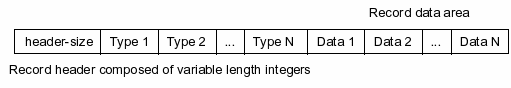
\includegraphics[scale=0.7]{images/recordformat.png}
	\caption{Database record format \citep{sqliteray}}
	\label{fig:sqlite_record_format}
\end{figure}

The cell header is made up of \textit{N + 1} varints where \textit{N} is the number of values in the record. The first varint is the number of bytes in the header, and the following \textit{N}, the record types.
\\\\
As varints can be between 1 - 9 bytes it is important to keep track of the varints size. To count the number of values in the record. For example, if there are \textit{N} values, and the number of bytes as 8. This could mean there are 8 small values, or 1 large value, or anywhere in between. The different value types can be seem below in Table~\ref{tbl:cell_header_record_types} 

\begin{longtable}[h]{| c | c| p{5cm} |}
		\hline
			\textbf{Header Value} & \textbf{Byte Size} & \textbf{Description} \\ 
		\hline
		\endhead
			0 & 0 & Null \\
		\hline
			1 & 1 & 1 byte signed integer \\
		\hline
			2 & 2 & 2 byte signed integer \\
		\hline
			3 & 3 & 3 byte signed integer \\
		\hline
			4 & 4 & 4 byte signed integer \\
		\hline
			5 & 6 & 6 byte signed integer \\
		\hline
			6 & 8 & 8 byte signed integer \\
		\hline
			7 & 8 & 8 byte IEEE floating point \\
		\hline
			8 & 0 & Value 0, Schema 4 or greater only \\
		\hline
			9 & 0 & Value 1, Schema 4 or greater only \\
		\hline
			10,11 & 0 & Reserved for expansion \\
		\hline
			$\geq$ 12 and even & \textit{(N-12)/2} & BLOB of size textit{(N-12/2)} long \\
		\hline
			$\geq$ 13 and odd & \textit{(N-13)/2} & String of size \textit{(N-13/2)} long \\
		\hline
	\caption{Database record cell types}
	\label{tbl:cell_header_record_types}
\end{longtable}

The cell content as shown in figure~\ref{fig:sqlite_record_format} follows the same format layout in the header, with the content size and type specified in table~\ref{tbl:cell_header_record_types}. Where the size is 0 there is no varint to read from the data section and should be skipped.

\subsubsection{Root B-Tree and Schema Table}
\label{subsubsec:schema_table}

As mentioned in section~\ref{subsubsec:sqlite_page_hader} following the SQLite header is the root B-Tree. The root B-Tree is one of the Table B-Trees with a defined payload format ( section~\ref{subsubsec:record_format}). This B-Tree payload contains pointer / page numbers to all the other pages in the file. It is referred to as the "sqlite\verb|_|master" table. Without parsing it properly you will only be able to access the "sqlite\verb|_|master" table.
\\\\
In some of the test databases, the root page was an Interior Table B-Tree, so going by page numbers in order to find the schema table is a bad idea. The Table~\ref{tbl:schema_table} below shows the payload / record layout of the "sqlite\verb|_|master" table.

\begin{longtable}[h]{| c | c| p{10cm} |}
		\hline
			\textbf{Field type} & \textbf{Field} & \textbf{Description} \\ 
		\hline
		\endhead
			Text & Type & The type of link: 'table', 'index', 'view', or 'trigger' \\
		\hline
			Text & Name & Name of the object / table, including constraints \\
		\hline
			Text & Table Name & Table Name \\
		\hline
			Integer & Root page & Root page number of this item \\
		\hline
			Text & SQL & Sql command used to create this object. \\
		\hline
	\caption{Schema table layout}
	\label{tbl:schema_table}
\end{longtable}

In order to tell if the current page is a table, the first column, should contain one of the four types, mentioned in the above table. Then read the page number in the fourth column to find the content for that table. Much like the right child pointer mentioned in section~\ref{subsubsec:btree_header} this is the page number of the child not a pointer.

\subsubsection{Parsing the file}
\label{subsubsec:parsing the file}

In order to parse the database file. The first thing would be to read in the header (section~\ref{subsubsec:sqlite_page_hader} ) then read in the root page(s) ( section~\ref{subsubsec:schema_table} ), and follow the page numbers to all the other table root pages, then start parsing them until all paths have been followed. This format leans towards recursion rather than iteration although both are possible.
